\documentclass{article}
\usepackage{eason}

\usepackage{pdfpages}

\usepackage[a4paper, margin=1in]{geometry}

\usepackage{lipsum}
\usepackage{multicol}

\newcommand{\DATE}{dummyDate}
\newcommand{\COMMITSHA}{dummySHA}

\title{TMUA Lecture 1 -- Basic Algebra}
\author{Eason Shao}
\date{v.\DATE.\COMMITSHA}

\begin{document}
\maketitle

\tableofcontents

\section{Factorisation Formulae}
\subsection{General}
\[
    \pqty{x \pm y}^2 = x^2 \pm 2xy + y^2, \quad \pqty{x \pm y}^3 = x^3 \pm 3 x^2 y + 3 x y^2 \pm y^3.
\]

\[
    x^2 - y^2 = \pqty{x + y} \pqty{x - y}.
\]

\[
    x^3 \pm y^3 = \pqty{x \pm y} \pqty{x^2 \mp xy + y^2}.
\]

\begin{example}
    Factorise \(x^4 - y^4\).
\end{example}

\begin{example}
    Factorise \(x^4 + 4 y^4\).
\end{example}

\begin{problem}
    When can \(x^n + y^n\) be factorised into a product of a linear factor and some other polynomial? What about \(x^n - y^n\)?
\end{problem}

\subsection{Binomial Theorem(s)}
The \textbf{binomial theorem} is a systematic way to expand expressions of the form \(\pqty{a + b}^n\) where \(n \in \NN\). With the notation
\[
    \binom{n}{k} = \frac{n!}{k! \pqty{n - k}!},
\]
we have
\[
    \pqty{a + b}^n = \sum_{k = 0}^{n} \binom{n}{k} a^k b^{n - k}.
\]

Written out in full, it reads
\[
    \pqty{x + y}^n = \binom{n}{0} x^n y^0 + \binom{n}{1} x^{n - 1} y^1 + \cdots + \binom{n}{n - 1} x^1 y^{n - 1} + \binom{n}{n} x^0 y^n.
\]

\begin{example}[TMUA 2016 P1 Q1]
    It is given that the expansion of \(\pqty{ax + b}^3\) is \(8 x^3 - p x^2 + 18 x - 3 \sqrt{3}\), where \(a\), \(b\) and \(p\) are real constants. What is the value of \(p\)?
\end{example}

\begin{example}[TMUA 2017 P1 Q13]
    In the expansion of \(\pqty{a + bx}^5\) the coefficient of \(x^4\) is \(8\) times the coefficient of \(x^2\).

    Given that \(a\) and \(b\) are non-zero positive integers, what is the smallest possible value of \(a + b\)?
\end{example}

It is worth noting that the binomial coefficient has special cases of
\[
    \binom{n}{0} = 1, \quad \binom{n}{1} = n, \quad \binom{n}{2} = \frac{n \pqty{n - 1}}{2};
\]
and there is a symmetry of
\[
    \binom{n}{k} = \binom{n}{n - k}.
\]  

\textbf{Newton's Binomial Theorem} extends this to the form \(\pqty{1 + x}^{\alpha}\) where \(\alpha \in \RR\) and \(\abs{x} < 1\). It states that
\[
    \pqty{1 + x}^{\alpha} = 1 + \alpha x + \frac{\alpha \pqty{\alpha - 1}}{2} x^2 + \frac{\alpha \pqty{\alpha - 1} \pqty{\alpha - 2}}{3!} x^3 + \cdots + \frac{\alpha \pqty{\alpha - 1} \cdots \pqty{\alpha - n + 1}}{n!} x^n + \cdots
\]
and note here that the sum does not terminate.

\begin{example}[TMUA 2016 P1 Q19]
    The coefficient of \(x^3\) in the expansion of \(\pqty{1 + 2x + 3 x^2}^6\) is equal to twice the coefficient of \(x^4\) in the expansion of \(\pqty{1 - a x^2}^5\). Find all possible values of the constant \(a\).
\end{example}

\begin{problem}
    Try proving the binomial theorem. Hint: prove and use the identity
    \[
        \binom{n + 1}{k} = \binom{n}{k} + \binom{n}{k - 1}.
    \]  
\end{problem}

\section{Exponents}

\[
    a^b a^c = a^{b + c}, \quad \frac{a^b}{a^c} = a^{b - c};
\]
\[
    \pqty{a^b}^c = a^{bc}, \quad \pqty{ab}^p = a^p b^p;
\]
\[
    a^{-p} = \frac{1}{a^p}, \quad a^{\frac{1}{p}} = \sqrt[p]{a};
\]
\[
    a^0 = 1, \quad a^1 = a, \quad a^{-1} = \frac{1}{a}.
\]

\begin{example}[TMUA 2016 P1 Q11]
    The real roots of the equation \(4^{2x} + 12 = 2^{2x + 3}\) are \(p\) and \(q\), where \(p > q\). Find \(p - q\).
\end{example}

\begin{example}[TMUA 2017 P1 Q14]
    The solution of the simultaneous equations
    \begin{align*}
        2^x + 3 \times 2^y &= 3 \\
        2^{2x} - 9 \times 2^{2y} &= 6
    \end{align*}
    is \(\pqty{x, y} = \pqty{p, q}\). Find the value of \(p - q\).
\end{example}

\begin{problem}
    What are the restrictions to the \(a, b, c, p\) above?
\end{problem}

Do not worry too much if the power is irrational (e.g. \(2^{\sqrt{2}}\)), or if the base is negative and the power is non-integer (e.g. \(\pqty{-64}^{\frac{1}{2}}\)), or if both occur at the same time (e.g. \(\pqty{-1}^{\pi}\)).

\section{Logarithms}

For \(a > 0, a \neq 1\) and \(c > 0\), the \textbf{logarithm} base-\(a\) of \(c\) is defined as the unique \(b \in \RR\) such that \(a^b = c\).
\[
    a^b = c \iff b = \log_a c.
\]  

Laws of logarithms can be deduced from laws of indices:
\[
    \log_a x + \log_a y = \log_a \pqty{xy}, \quad \log_a x - \log_a y = \log_a \pqty{\frac{x}{y}};
\]
\[
    k \log_a x = \log_a \pqty{x^k}, \quad \frac{1}{k} \log_a x = \log_a \pqty{x^{\frac{1}{k}}};
\]
\[
    \log_a 1 = 0, \quad \log_a a = 1, \quad \log_a \frac{1}{a} = -1.
\]

\textbf{Change of base formula.} for \(a, b, c > 0, a \neq 1, c \neq 1\),
\[
    \log_a b = \frac{\log_c b}{\log_c a}.
\]

\begin{problem}
    Is their an equivalent version of change of base formula in exponentiation? How to prove the logarithm change of base formula?
\end{problem}

\begin{example}[TMUA 2016 P1 Q16]
    Given the simultaneous equations
    \begin{align*}
        \log_{10} 2 + \log_{10} \pqty{y - 1} &= 2 \log_{10} x \\
        \log_{10} \pqty{y + 3 - 3x} &= 0,
    \end{align*}
    find the values of \(y\).
\end{example}

\section{Surds}

Simplifying square roots: \(\sqrt{a^2 b} = \abs{a} b\). \textbf{Do not forget to check whether the thing moved outside is positive or not.}

Morale: \(\pqty{a + \sqrt{b}}\) multiplied with \(\pqty{a - \sqrt{b}}\) (its \textbf{conjugate surd}) gives \(a^2 - b\), a rational.

Application: rationalisation of denominators
\[
    \frac{c}{a + \sqrt{b}} = \frac{c}{a + \sqrt{b}} \cdot \frac{a - \sqrt{b}}{a - \sqrt{b}} = \frac{c \pqty{a - \sqrt{b}}}{a^2 - b}.
\]

Quick trick:
\[
    \sqrt{\frac{1}{a}} = \frac{\sqrt{a}}{a}.
\]

\textbf{Square roots are never negative.}

\begin{example}
    Simplify the nested square roots \(\sqrt{49 \pm 12 \sqrt{5}}\) and \(\sqrt{7 \pm 2 \sqrt{10}}\).
\end{example}

\begin{example}[TMUA 2017 P2 Q8]
    Which one of the following numbers is smallest in value?

    \begin{enumerate}
        \item \(\log_2 7\)
        \item \(\pqty{2^{-3} + 2^{-2}}^{-1}\)
        \item \(2^{\flatfrac{\pi}{3}}\)
        \item \(\dfrac{1}{4\pqty{\sqrt{2} - 1}^3}\)
        \item \(4 \sin^2 \pqty{\flatfrac{\pi}{4}}\)
    \end{enumerate}
\end{example}

\begin{problem}
    Find what is wrong with the following proof.

    \[
        1 = \sqrt{1} = \sqrt{\pqty{-1} \pqty{-1}} = \sqrt{-1} \sqrt{-1} = i^2 = -1.
    \]  
\end{problem}

\section{Quadratic Functions and Quadratic Equations}
\subsection{Quadratic Formula}

Consider the equation in \(x\): \(a x^2 + bx + c = 0\) (\(a \neq 0\)).

The \textbf{quadratic formula} reads:
\[
    x = \frac{-b \pm \sqrt{b^2 - 4ac}}{2a}
\]
where \(\Delta = b^2 - 4ac\) is the \textbf{discriminant}.

Proof is by completing the square.

\begin{align*}
    a x^2 + bx + c &= a \pqty{x^2 + \frac{b}{a} x + \frac{b^2}{4 a^2}} + c - \frac{b^2}{4a} \\
    &= a \pqty{x + \frac{b}{2a}}^2 + \frac{4ac - b^2}{4a}.
\end{align*}

This means the vertex of the graph (the optimum) has coordinates
\[
    \pqty{- \frac{b}{2a}, \frac{4ac - b^2}{4a}}.
\]

\subsection{Discriminant}
The \textbf{discriminant} tells us about the roots of the equation.
\begin{itemize}
    \item If \(\Delta > 0\), then the equation has two distinct real roots.
    \item If \(\Delta = 0\), then the equation has two repeated (equal) real roots.
    \item If \(\Delta < 0\), then the equation has no real roots. (The roots are complex conjugates.)
\end{itemize}

The discriminant (together with the leading factor) also tells us whether the graph of the quadratic lies above/below or intersects the \(x\)-axis.

\begin{example}[TMUA 2017 P2 Q14]
    The diagram in \autoref{fig:tmua-2017-p2-q14} shows the graph of \(y = x^2 - 2bx + c\). The vertex of this graph is at the point \(P\).

    Which one of the following could be the graph of \(y = x^2 - 2Bx + c\), where \(B > b\)?
\end{example}

\begin{figure}[h!]
    \centering
    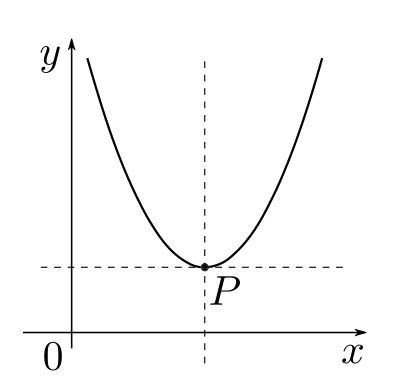
\includegraphics[width=0.3\linewidth]{tmua-2017-p2-q14-img1}
    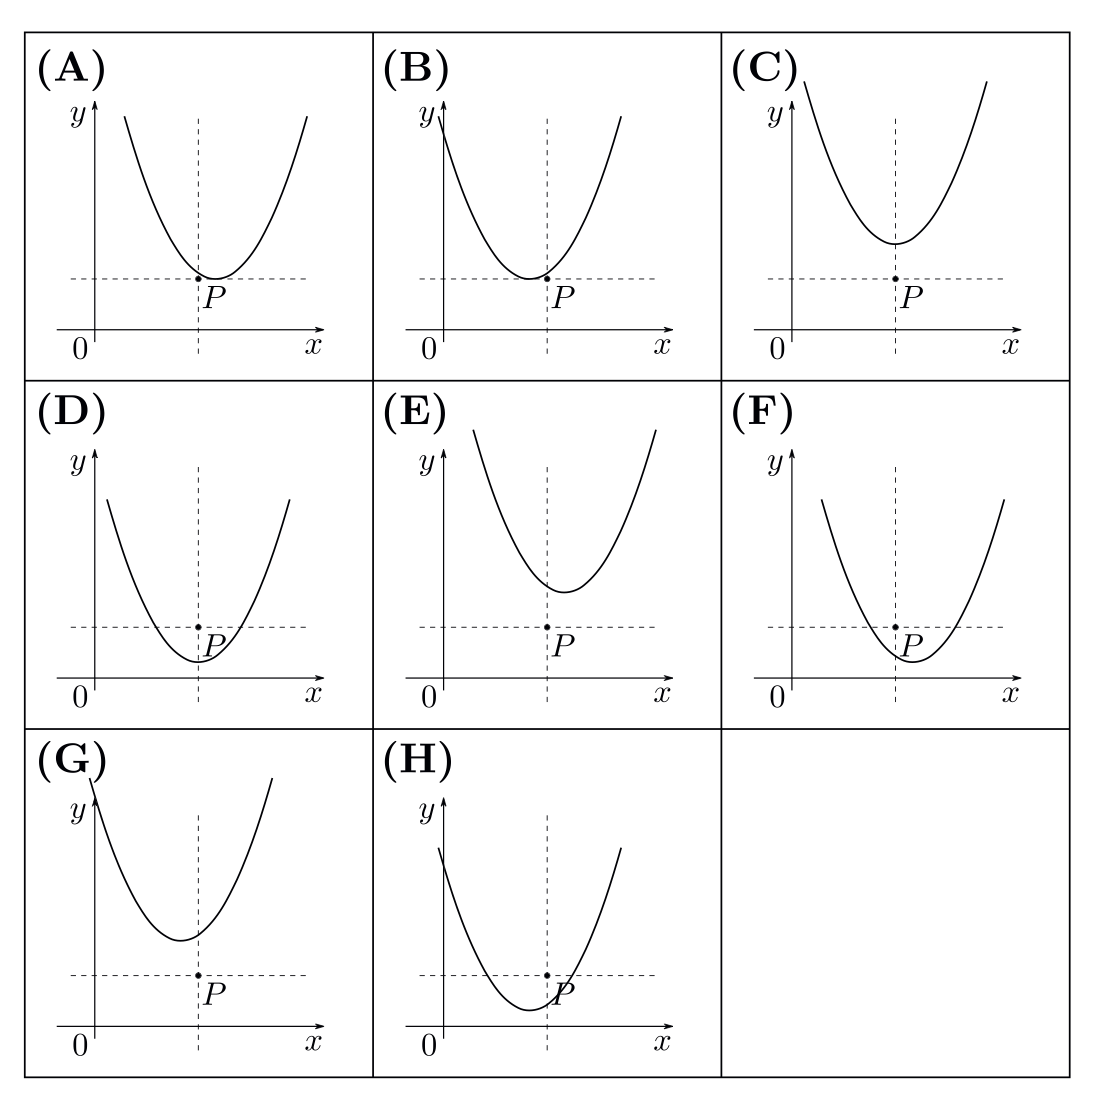
\includegraphics[width=0.7\linewidth]{tmua-2017-p2-q14-img2}
    \caption{TMUA 2017 P2 Q14}
    \label{fig:tmua-2017-p2-q14}
\end{figure}

\subsection{Vieta's Theorem}
\textbf{Vieta's Theorem} states the two roots satisfy
\[
    x_1 + x_2 = - \frac{b}{a}, \quad x_1 x_2 = \frac{c}{a}.
\]

Proof is by quadratic formula (very disgusting), or by factorisation. We have
\[
    a x^2 + bx + c = a \pqty{x - x_1} \pqty{x - x_2}
\]
and expanding the brackets gives us the result.

\begin{example}
    Let \(x_1, x_2\) be the two real roots for the equation \(x^2 - 4x + 1 = 0\). Find:
    \begin{itemize}
        \item \(x_1^2 + x_2^2\);
        \item \(x_1^3 + x_2^3\);
        \item \(x_1^4 + x_2^4\).
    \end{itemize}
\end{example}

\begin{example}
    Let \(x_1, x_2\) be the two real roots for the equation \(x^2 - \pqty{k - 2} x + \pqty{k^2 + 3k + 10} = 0\). Find the largest values of \(x_1^2 + x_2^2\).
\end{example}

\begin{example}[TMUA 2016 P2 Q15]
    Consider the quadratic \(f\pqty{x} = x^2 - 2px + q\) and the statement \(f\pqty{x} = 0\) has two real roots whose difference is greater than \(2\) and less than \(4\).

    Which one of the following statements is true if and only if the above statement is true?

    \begin{enumerate}
        \item \(q < p^2 < q + 4\)
        \item \(\sqrt{q + 1} < p < \sqrt{q + 4}\)
        \item \(q - 3 \leq p^2 - 4 \leq q\)
        \item \(q < p^2 - 1 < q + 3\)
        \item \(q - 2 < p^2 - 3 < q + 2\)
    \end{enumerate}
\end{example}

\subsection{Alternative Forms of Quadratics}
It is often more useful to look at a quadratic using its alternate forms:
\begin{itemize}
    \item \(a \pqty{x - p}^2 + q\) which tells us about its vertex \(\pqty{p, q}\);
    \item \(a \pqty{x - x_1} \pqty{x - x_2}\) which tells us about its roots \(x_{1, 2}\).
\end{itemize}

\section{Simultaneous Equations}

Key strategies: change of variable, elimination, reduction of power.

If you have a equation in \(x\) and \(y\) and you want to find \(y\), express \(y\) in terms of \(x\) and substitute in (this is called \textbf{elimination}).

If the equation relates multiple powers of \(x\), then substituting other occurrences of e.g. \(x^2\) with lower powers is called \textbf{reduction of power}.

\section{Inequalities}
\subsection{Simple Inequalities}
\[
    a > b, b > c \implies a > c; \quad a > b \implies a + c > b + c;
\]
\[
    a > b, c > 0 \implies ac > bc; \quad a > b, c < 0 \implies ac < bc;
\]
\[
    a > b, c > d \implies a + c > b + d; \quad a > b > 0, c > d > 0 \implies ac > bd.
\]

\begin{example}[TMUA 2017 P2 Q13]
    The positive real numbers \(a \times 10^{-3}\), \(b \times 10^{-2}\) and \(c \times 10^{-1}\) are each in standard form, and
    \[
        \pqty{a \times 10^{-3}} + \pqty{b \times 10^{-2}} = \pqty{c \times 10^{-1}}.
    \]

    Which of the following statements must be true?
    \begin{enumerate}
        \item \(a > 9\)
        \item \(b > 9\)
        \item \(a < c\)
        \item \(b < c\)
    \end{enumerate}
\end{example}

\subsection{Quadratic Inequalities}
Quadratic inequalities can be solved by considering the leading coefficient and the discriminant. The most useful way to demonstrate is to sketch a graph.

\begin{example}[TMUA 2017 P1 Q19]
    The set of solutions to the inequality \(x^2 + bx + c < 0\) is the interval \(p < x < q\), where \(b, c, p\) and \(q\) are real constants with \(c < 0\). In terms of \(p, q\) and \(c\), find the set of solutions to the inequality \(x^2 + bcx + c^3 < 0\).
\end{example}

\subsection{Factorisable Inequalities}
More complicated inequalities of the form
\[
    f_1\pqty{x} f_2\pqty{x} \cdots f_m\pqty{x} > 0
\]
can be solved by considering the critical values of \(f_i\) (i.e. solving \(f_i\pqty{x} = 0\)) and considering the signs in the respecting intervals split up by such critical values.

\begin{example}
    Solve the inequality \(\pqty{x - 2} \pqty{x + 1} \pqty{x - 1} > 0\).
\end{example}

\begin{example}
    Solve the inequality \(\pqty{x - 2}^2 \pqty{x + 1} < 0\).
\end{example}

\begin{example}[TMUA 2016 P2 Q8]
    A region is defined by the inequalities \(x + y > 6\) and \(x - y > -4\). Consider the three statements:
    \begin{enumerate}
        \item \(x > 1\)
        \item \(y > 5\)
        \item \(\pqty{x + y} \pqty{x - y} > -24\)
    \end{enumerate}


    Which of the above statements is/are true for every point in the region?
\end{example}

\begin{example}[TMUA 2017 P2 Q5]
    \(S\) is the complete set of values of \(x\) which satisfy \textbf{both} the inequalities \(x^2 - 8x + 12 < 0\) \textbf{and} \(2x + 1 > 9\). It can also be represented as a single inequality. Which one of the following single inequalities represents the set \(S\)?

    \begin{enumerate}
        \item \(\pqty{x^2 - 8x + 12} \pqty{2x + 1} < 0\)
        \item \(\pqty{x^2 - 8x + 12} \pqty{2x + 1} > 0\)
        \item \(x^2 - 10 x + 24 < 0\)
        \item \(x^2 - 10 x + 24 > 0\)
        \item \(x^2 - 6 x + 8 < 0\)
        \item \(x^2 - 6 x + 8 > 0\)
        \item \(x < 2\)
        \item \(x > 6\)
    \end{enumerate}
\end{example}

\section{Polynomials}
\subsection{Definition}
A \textbf{polynomial} is of the form
\[
    a_n x^n + a_{n - 1} x^{n - 1} + \cdots + a_1 x + a_0
\]
where \(n \geq 0\) is a natural number. Such \(n\) is called the \textbf{degree} of a polynomial. \(a_n, a_{n - 1}, \ldots, a_1, a_0\) are the \textbf{coefficients} of the polynomial. (We assume that they are real).

\subsection{Polynomial Division and Factor Theorem}
\textbf{Polynomial division/remainder theorem} (Euclidean division) states that for any polynomial \(P\) (the polynomial to be divided) and \(D \neq 0\) (the \textbf{divisor}), there are two polynomials \(Q\) (the \textbf{quotient}) and \(R\) (the \textbf{remainder}), such that
\[
    P \pqty{x} = Q \pqty{x} D\pqty{x} + R \pqty{x}
\]
where \(\deg R < \deg D\).

\textbf{Long division} and \textbf{synthetic division} are computational methods to divide polynomials.

\begin{example}
    Divide the polynomial \(\pqty{x^4 + 2 x^3 + 3x + 5}\) by \(\pqty{x^2 + 2x + 1}\).
\end{example}

\textbf{Factor theorem} states that the remainder of a polynomial \(P\) upon division by \(\pqty{x - a}\) is a constant given by \(P\pqty{a}\).

\begin{proof}
    Write \(P\pqty{x} = \pqty{x - a} D\pqty{x} + R\pqty{x}\) and observe \(R\) has degree less than \(1\), hence constant. Plug in \(x = a\).
\end{proof}

\begin{example}[TMUA 2016 P1 Q2]
    The expression \(3 x^3 + 18 x^2 + 8x + a\), where \(a\) is a constant, has \(\pqty{x + 2}\) as a factor. Factorise this expression.
\end{example}

\begin{example}[TMUA 2016 P1 Q4]
    When \(\pqty{3 x^2 + 8x - 3}\) is multiplied by \(\pqty{px - 1}\) and the resulting product is divided by \(\pqty{x + 1}\), the remainder is \(24\). What is the value of \(p\)?
\end{example}

\subsection{Roots of Polynomials}
\textbf{Fundamental Theorem of Algebra} states that for any degree-\(n\) complex polynomial \(P\pqty{x}\), it has \(n\) complex roots (including repeats), and hence can be factorised in the form
\[
    P\pqty{x} = a_n \pqty{x - x_1} \pqty{x - x_2} \cdots \pqty{x - x_n}.
\]

If \(P\) is a real polynomial, the roots \(x_1, \ldots, x_n\) may be complex, but complex roots come in conjugate pairs, so it can be factorised into linear and quadratic factors.

In practice, using this factorisation to determine how many real roots a polynomial has is very impracticable. Therefore, we analyse its stationary points and its increasing/decreasing property (i.e. analyse the sign of \(P'\pqty{x}\)) to determine the number of roots it has.

Recall the \textbf{intermediate value theorem} states that if \(\functiondomain{f}{\ccintv{a}{b}}{\RR}\) is continuous, with \(f\pqty{a} < 0\) and \(f\pqty{b} > 0\), then there is some \(c \in \oointv{a}{b}\) such that
\[
    f\pqty{c} = 0.
\]

Together with monotonicity, we may assert that such \(c\) is in fact unique.

\begin{example}[TMUA 2016 P1 Q13]
    How many real roots does the equation \(3 x^5 - 10 x^3 - 120 x + 30 = 0\) have?
\end{example}

\begin{example}[TMUA 2016 P2 Q14]
    Let \(f\pqty{x} = a x^4 + b x^3 + c x^2 + d x + e\), where \(a, b, c, d\) and \(e\) are real numbers. Suppose \(f\pqty{x} = 1, 2, 3, 4\) has \(p, q, r, s\) solutions, respectively, which one of the following is \emph{not} possible?
    \begin{enumerate}
        \item \(\pqty{p, q, r, s} = \pqty{1, 2, 4, 3}\),
        \item \(\pqty{p, q, r, s} = \pqty{1, 3, 2, 4}\),
        \item \(\pqty{p, q, r, s} = \pqty{1, 4, 3, 2}\),
        \item \(\pqty{p, q, r, s} = \pqty{2, 4, 3, 1}\),
        \item \(\pqty{p, q, r, s} = \pqty{4, 3, 2, 1}\).
    \end{enumerate}
\end{example}

\begin{example}[TMUA 2017 P2 Q19]
    Which one of the following is a sufficient condition for the equation \(x^3 - 3 x^2 + a = 0\), where \(a\) is a constant, to have exactly one real root?
    \begin{enumerate}
        \item \(a > 0\)
        \item \(a \leq 0\)
        \item \(a \geq 4\)
        \item \(a < 4\)
        \item \(\abs{a} > 4\)
        \item \(\abs{a} \leq 4\)
        \item \(a = \frac{9}{4}\)
        \item \(\abs{a} = \frac{3}{2}\)
    \end{enumerate}
\end{example}

\end{document}